\documentclass[12pt,a4paper]{report}
\usepackage[utf8]{inputenc}
\usepackage{cite}
\usepackage{float}
\usepackage{csquotes}
\usepackage[english]{babel}
\usepackage{multirow}
\usepackage[normalem]{ulem}
\useunder{\uline}{\ul}{}
\usepackage{hyperref}
\usepackage{graphicx}
\usepackage[T1]{fontenc}
\usepackage{listings}
\usepackage{xcolor}
\usepackage{subfig}
\usepackage{geometry}
\usepackage{xcolor}
\usepackage{graphicx}
\usepackage{float}
\usepackage{tabularx} % Adaugat pachetul tabularx
\usepackage{changepage} % Adaugă pachetul pentru mediu adjustwidth
\usepackage{booktabs}
\usepackage{enumitem}

\lstdefinestyle{bashstyle}{
    language=bash,
    basicstyle=\small\ttfamily,
    backgroundcolor=\color{gray!10},
    frame=tb,
    framerule=0pt,
    aboveskip=3mm,
    belowskip=3mm,
    showstringspaces=false,
    columns=flexible,
    numbers=none,
    keywordstyle=\color{blue},
    commentstyle=\color{gray},
    stringstyle=\color{green!60!black},
    breaklines=true,
    breakatwhitespace=true,
    tabsize=4
}

\renewcommand\thesection{\arabic{section}.} 
\renewcommand\thesubsection{\arabic{section}.\arabic{subsection}}
\renewcommand\thesubsubsection{\thesubsection.\arabic{subsubsection}} % Subsubsection numbering format


\title{Verificarea rețelelor neuronale folosind alpha\textunderscore beta\textunderscore crown și NeuralSat pentru benchmark-ul cGan al competiției VNN-Comp 2023}
\author{ Diaconu Laura\\ Domșa Emanuel\\Laptedulce Anastasia \\ Morariu Ioana-Alexandra \\ Romaneț Rareș}

\date{}


\begin{document}
\maketitle


\begin{abstract}
In this paper, we attempted to reproduce the results from the VNNCOMP-2023 competition, specifically focusing on the alpha-beta-CROWN and Marabou tools applied to the cGAN benchmark within the same competition. The paper begins with a brief description of how cGAN neural networks operate, followed by a characterization of the dataset and the steps taken to install the tools and run them. We analyzed the data obtained from the runs and compared them with those obtained in the competition. \textbf{TO DO: Maybe add a brief ideea of the conlusions made after analysis}
\end{abstract}
\tableofcontents
\newpage

%%%%%%%%%%%%%%%%%%%%%%%%%%%%%%%%%%%%%%%%%%%%%%%%%%%%%%%%%%%%%%%%%%%%%%%%%%%%
\section{Introducere - Funcționarea rețelei neuronale}
\hspace{0.5 cm} Verificarea rețelelor neuronale este un proces esențial în dezvoltarea și implementarea acestor modele avansate. Această practică reprezintă un pilon fundamental din mai multe motive cheie.

În primul rând, corectitudinea și fiabilitatea rețelelor neuronale sunt imperative. Acestea sunt utilizate într-o varietate de domenii, de la medicină și tehnologie la securitate cibernetică și vehicule autonome. Verificarea asigură că aceste rețele operează conform așteptărilor, furnizând rezultate precise și de încredere într-o gamă largă de scenarii.

Siguranța este un alt aspect crucial. În aplicații critice, cum ar fi cele medicale sau cele legate de siguranța vehiculelor, erorile în funcționarea rețelelor neuronale pot avea consecințe grave. Verificarea acestora este vitală pentru a identifica și a remedia potențialele vulnerabilități care ar putea compromite siguranța sistemelor.

De asemenea, verificarea rețelelor neuronale ajută la prevenirea bias-ului și discriminării. Aceste rețele pot fi susceptibile la prejudecăți încorporate din datele de antrenament. Prin testare și evaluare riguroasă, se poate identifica și corecta aceste bias-uri pentru a asigura obiectivitate și echitate în rezultatele furnizate.
%%%%%%%%%%%%%%%%%%%%%%%%%%%%%%%%%%%%%%%%%%%%%%%%%%%%%%%%%%%%%%%%%%%%%%%%%%%%



%%%%%%%%%%%%%%%%%%%%%%%%%%%%%%%%%%%%%%%%%%%%%%%%%%%%%%%%%%%%%%%%%%%%%%%%%%%%
\section{Caracterizarea setului de date}
Benchmark-ul cGAN aparține mulțimii de benchmark-uri din cadrul competiției VNN-COMP 2023 \cite{vnncompBenchmarks}. Acesta conține o rețea de tip generativă adversarială condiționată și un set de specificații. Benchmark-ul este folosit pentru a verifica corectitudinea și robustețea rețelei pe care o conține. În cadrul set-ului de date, există două tipuri de fișiere: .onnx (Open Neural Network Exchange) și .vnnlib. În fișierele .onnx sunt reprezentate rețele neuronale, acestea conțin informații necesare pentru a executa modelul neuronal. Fișierele .vnnlib conțin specificațiile ce trebuie respectate de rețeaua neuronală, astfel încât aceasta să fie corectă și robustă.

Atât fișierele .onnx cât și .vnnlib au o denumire sugestivă care să indice informații despre conținutul acestora.
\begin{figure}[ht]
\begin{tabular}{cc}
\hspace{-2cm} \subfloat[Fișiere .onnx]{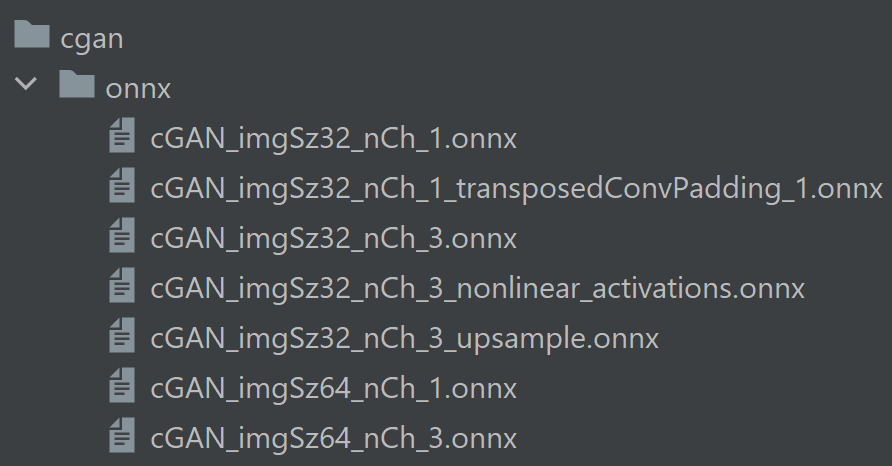
\includegraphics[width=7.5cm]{imagini/caracterizareSetDate/onnx.png}} &
\hspace{-0.5cm} \subfloat[Fișiere .vnnlib]{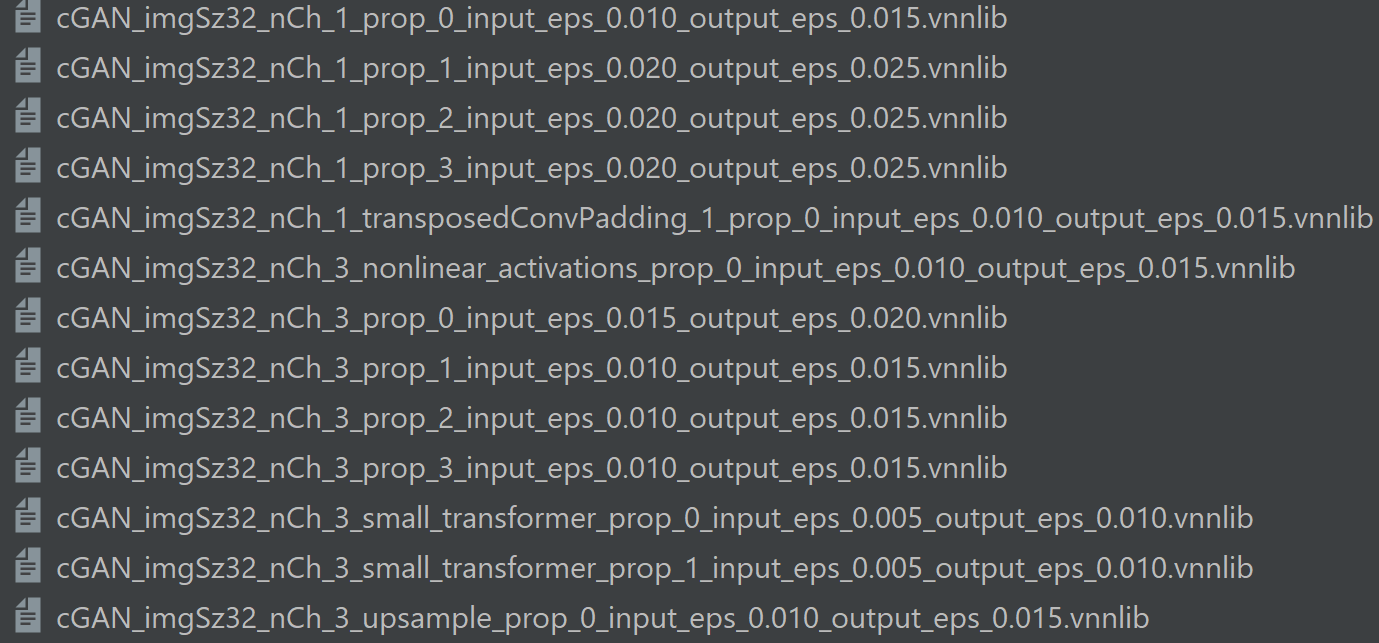
\includegraphics[width=10cm]{imagini/caracterizareSetDate/vnnlib.png}}
\end{tabular}
\caption{Fișierele benchmark-ului cGAN}
\end{figure}
\begin{itemize}
  \item \textit{CGan} - tipul de rețea neurală, în acest caz, o rețea generatoare adversarială condiționată.
  
  \item \textit{imgSz32} - dimensiunea imaginei generate, în acest caz, o dimensiune de 32x32 pixeli.

  \item \textit{nCh\_1} - numărul de canale de culoare utilizate în imaginile de intrare sau de ieșire ale rețelei.
  
  \item \textit{prop\_0} - parametru/proprietate specifică a imaginei

  \item \textit{input\_eps\_0} - valoare epsilon utilizată peste datele de intrare ale rețelei.
  
  \item \textit{output\_eps\_0.015} -  valoare epsilon utilizată peste datle de ieșire a rețelei.


  \item \textit{transportedConvPadding\_1} - tip specific de convoluție a rețelei.
  
  \item \textit{nonlinear\_activations} - rețeaua conține funcții de activare non-liniare între straturi.

  \item \textit{upsample} - modelul neuronal efectuează operații de upsampling, care sunt utilizate pentru a mări dimensiunea spațială a imaginilor sau a datelor. Aceasta poate fi utilă în cazul modelelor generatoare pentru a genera imagini de rezoluție mai mare sau în alte scenarii în care este necesară mărirea dimensiunii datelor.
  
\end{itemize}

Toate fisierele .vnnlib au același conținut, diferențiindu-se prin valorile datelor.

\begin{lstlisting}[language=Lisp, caption={Exemplu de cod SMT-LIB din fisierele vnnlib}, label={lst:smtlib}, basicstyle=\scriptsize\ttfamily]
(declare-const X_0 Real)
(declare-const X_1 Real)
(declare-const X_2 Real)
(declare-const X_3 Real)
(declare-const X_4 Real)

(declare-const Y_0 Real)

; Input constraints:
(assert (<= X_0 val_1_X0))
(assert (>= X_0 val_2_X0))

(assert (<= X_1 val_1_X1))
(assert (>= X_1 val_2_X1))

(assert (<= X_2 val_1_X2))
(assert (>= X_2 val_2_X2))

(assert (<= X_3 val_1_X3))
(assert (>= X_3 val_2_X3))

(assert (<= X_4 val_1_X4))
(assert (>= X_4 val_2_X4))

; Output constraints:
(assert (or
    (and (>= Y_0 val_1_Y0))
    (and (<= Y_0 val_2_Y0))
))

\end{lstlisting}

Luând în considerare succinta descriere a autorului benchmark-ului , din fișiere .vnnlib, am dedus următoarele:

\begin{itemize}
  \item \textit{X\_0} - reprezintă condiția de distanță ce este o variabilă cuprinsă între 0 și 1 și reprezintă normalizarea de la 0m la 30 m (de exemplu dacă condiția de distanță este 0,5, înseamnă că va fi generată o imagine ce are obstacolul la 0,5*30m=15m)
  
  \item \textit{$X\_1$ și până la $X\_4$} - reprezintă valorile vectorului de zgomot care controlează mediul
  
  \item \textit{$Y\_0$}  - reprezintă distanța dată de către generator
  
\end{itemize}
%%%%%%%%%%%%%%%%%%%%%%%%%%%%%%%%%%%%%%%%%%%%%%%%%%%%%%%%%%%%%%%%%%%%%%%%%%%%



%%%%%%%%%%%%%%%%%%%%%%%%%%%%%%%%%%%%%%%%%%%%%%%%%%%%%%%%%%%%%%%%%%%%%%%%%%%%
\section{Instalarea și rularea tool-urilor}
Pentru a efectua rularea benchmark-ului cGan, am selectat cu atenție tool-urile alpha-beta-CROWN și NeuralSAT, inițial verificând dacă acestea pot procesa setul de date specificat. Am făcut această selecție pentru a realiza o comparație între primul tool care a obținut un timp de verificare eficient în timpul competiției și al doilea tool care a înregistrat cel mai ineficient timp de verificare. Alegerea a fost orientată de dorința de a evalua performanțele și eficacitatea fiecărui tool în contextul benchmark-ului cGan.
    \subsection{alpha-beta-CROWN}
    Pentru a instala alpha\textunderscore beta\textunderscore CROWN am urmărit pașii de la capitolul \textit{Installation and Setup} din fișierul de READ.ME gasit pe link-ul de github al tool-ului \cite{read_abc.md}. 
Suplimentar pașilor din ghid, am clonat submodulul \textit{auto\textunderscore LIRPA} în interiorul directorului alpha-beta-CROWN. 
    \begin{lstlisting}[style=bashstyle]
    git clone https://github.com/Verified-
    Intelligence/auto_LiRPA.git alpha-beta-CROWN/auto_LiRPA
   \end{lstlisting}

Următorul pas efectuat ce nu se regăsește în ghid, a fost crearea directorului \texttt{vnncomp2023\_benchmarks} și clonarea repository-ului \cite{cganrepository} în interiorul acestuia. Ulterior, am modificat \textbf{root path-ului} în fișierul \texttt{cgan.yaml} conform locației reale a directorului \texttt{cgan}.

La rularea tool-ului ne-am confruntat cu o eroarea legată de lipsa librării \texttt{libcudnn\_cnn\_infer.so.8}. Adăugarea următoarei linii în fișierul \texttt{.bashrc} a rezolvat problema.
  \begin{lstlisting}[style=bashstyle]
    export LD_LIBRARY_PATH=/usr/lib/wsl/lib:$LD_LIBRARY_PATH
  \end{lstlisting}
  
Comanda de rularea a tool-ului este redată mai jos.
  \begin{lstlisting}[style=bashstyle]
    python abcrown.py --config exp_configs/vnncomp23/cgan.yaml
  \end{lstlisting}
In dependență de conținutul fișierului \textit{cgan.yaml}, respectiva comandă are output diferit.

Cel mai dificil pas a fost remedierea erorii legate de libraria libcudnn\textunderscore cnn\textunderscore infer.so.8., fiind si pasul care a durat cel mai mult timp. Am rezolvat aceasta eroare folosind multiple sugestii gasite pe diferite platforme online \cite{bashrcfix}.
    \subsection{NeuralSAT}
    \hspace{0.5 cm}
Pentru a putea interpreta datele rezultate le-am clasificat manual în tabel la fel ca și cele obținute folosind alpha-beta-CROWN. Câmpurile de tabel sunt identice cu cele de la alpha-beta-CROWN, singura excepție fiind ocurența a tipuri noi de rezultate, și anume:
\begin{itemize}
    \item \textbf{results (vnncomp2023/us)}: Poate avea valori sat/unsat/unknown/error; pentru \textbf{sat} și \textbf{unsat} interpretările sunt la fel ca și în cazul alpha-beta-CROWN, pentru \textbf{unknown} înseamnă că proprietatea nu a putut fi demonstrată, iar \textbf{error} rezultă atunci când a avut loc o eroare în timpul rulării tool-ului.
    Prima coloană cu rezultate reprezintă rezultatele obținute în competiție, iar a două coloană contine rezultatele obtinute de noi.
\end{itemize}

În tabelul \ref{fig:image2} se prezintă o analiză comparativă între rezultatele obținute în urma rulării proprii și cele obținute în cadrul competiției.

\begin{figure}[h]
\centering 
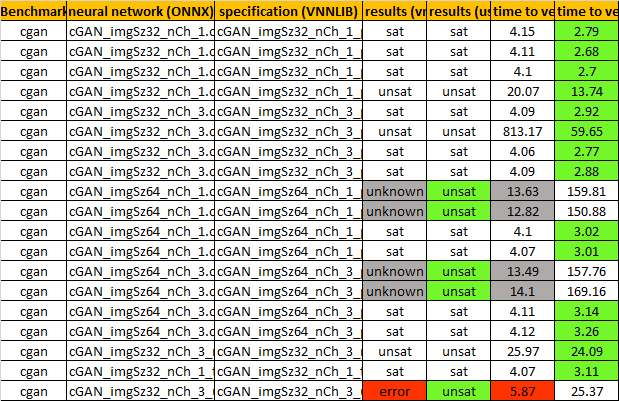
\includegraphics[width=0.8\linewidth]{imagini/interpretare rezultate/NeuralSAT_comp_vs_us.png}
\caption{Comparare rezultate NeuralSAT}
\label{fig:image2} 
\end{figure}
\

Comparând coloanele de \textit{results} am observat faptul că pentru toate instanțele am obținut valori satisfiabile sau nesatisfiabile. În schimb, competiția a obținut în cazul unor instanțe valori de \textit{unknown} si \textit{error}.

Graficul prezentat mai jos\ref{fig:image4}, evidențiază distribuirea timpilor de execuție pentru fiecare instanță în parte. În cadrul graficului de mai jos, se pot observa diferențele dintre timpii de execuție.
\begin{figure}[h]
\centering 
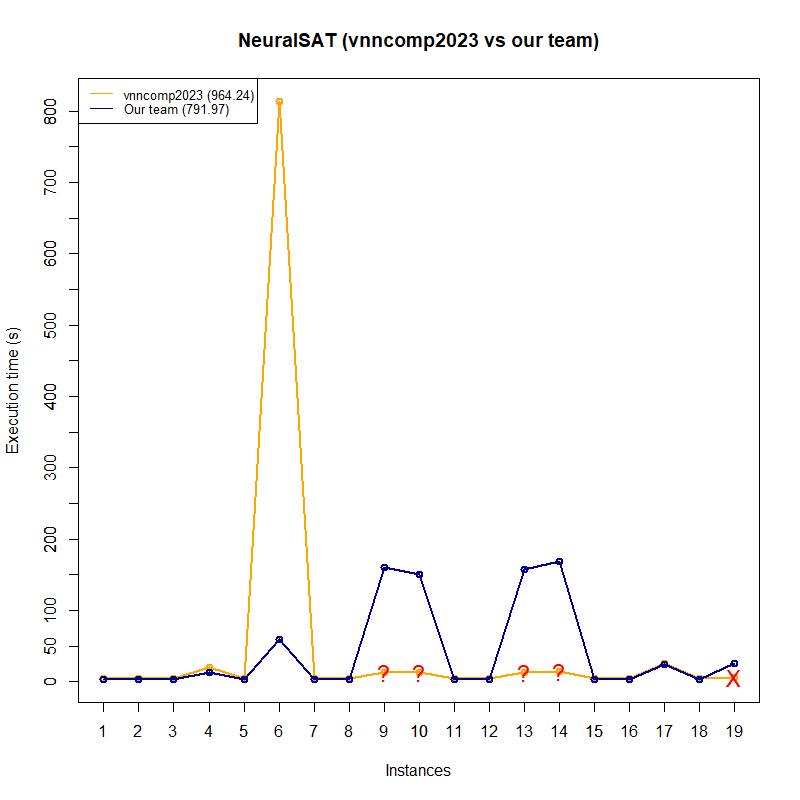
\includegraphics[width=0.8\linewidth]{imagini/interpretare rezultate/NeuralSAT_us_vs_vnncomp2023.png}
\caption{Comparare rezultate NeuralSAT}
\label{fig:image4} 
\end{figure}
\
%%%%%%%%%%%%%%%%%%%%%%%%%%%%%%%%%%%%%%%%%%%%%%%%%%%%%%%%%%%%%%%%%%%%%%%%%%%%



%%%%%%%%%%%%%%%%%%%%%%%%%%%%%%%%%%%%%%%%%%%%%%%%%%%%%%%%%%%%%%%%%%%%%%%%%%%%
\section{Interpretarea rezultatelor}
Pentru a efectua rularea benchmark-ului cGan, am selectat cu atenție tool-urile alpha-beta-CROWN și NeuralSAT, inițial verificând dacă acestea pot procesa setul de date specificat. Am făcut această selecție pentru a realiza o comparație între primul tool care a obținut un timp de verificare eficient în timpul competiției și al doilea tool care a înregistrat cel mai ineficient timp de verificare. Alegerea a fost orientată de dorința de a evalua performanțele și eficacitatea fiecărui tool în contextul benchmark-ului cGan.
    \subsection{alpha-beta-CROWN}
    În tabelul de mai jos se prezintă o analiză comparativă între rezultatele obținute în urma rulării proprii și cele obținute în cadrul competiției. Fișierele cu rezultatele rulărilor pot fi accesate la următoarele linkuri:
\href{https://docs.google.com/spreadsheets/d/1iGJHwePCzW0axJIwVes_eiN3R4ppvNu-ndrO_Fy5dL0/edit#gid=1265769327}{rezultate competiție }
\href{https://docs.google.com/spreadsheets/d/1kSxunni8qgQLT6ZkCRWvSO2VMy2Hz7qA/edit#gid=1476783028}{rezultate echipă}

\begin{figure}[h]
\centering 
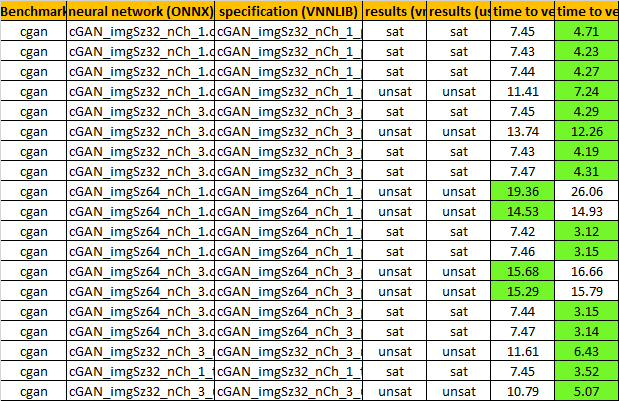
\includegraphics[width=0.8\linewidth]{imagini/interpretare rezultate/abC_comp_vs_us.png}
\caption{Rezultate alpha-beta-CROWN}
\label{fig:image1} 
\end{figure}

Din tabelul \ref{fig:image1}, este de notat faptul că pentru fiecare intrare, rezultatele(sat/unsat) au fost aceleași, atât pentru rezultatele rulării noastre, cât și pentru cele din competiție. Diferenta dintre competitie si echipa o constituie timpul de verificare. Timpul de verificare înregistrat al echipei este mai mic cu aproximativ 3 secunde pentru intrările unde rezultatul este satisfiabil. În schimb, pentru intrările cu rezultat nesatisfiabil timpul de verificare este considerabil mai mare.

Conform tabelului prezentat în \ref{fig:image1}, este de remarcat faptul că pentru fiecare intrare, rezultatele satisfiabil/nesatisfiabil) au fost aceleași, atât pentru rezultatele rulării proprii, cât și pentru cele din competiție. Diferența majoră între competiție și echipa noastră o constituie timpul de verificare. Timpul de verificare înregistrat al echipei noastre este mai mic cu aproximativ 3 secunde pentru intrările cu rezultat satisfiabil. În schimb, pentru intrările cu rezultat nesatisfiabil, timpul de verificare este considerabil mai mare.
    \subsection{NeuralSAT}
    \hspace{0.5 cm}
Pentru a putea interpreta datele rezultate le-am clasificat manual în tabel la fel ca și cele obținute folosind alpha-beta-CROWN. Câmpurile de tabel sunt identice cu cele de la alpha-beta-CROWN, singura excepție fiind ocurența a tipuri noi de rezultate, și anume:
\begin{itemize}
    \item \textbf{results (vnncomp2023/us)}: Poate avea valori sat/unsat/unknown/error; pentru \textbf{sat} și \textbf{unsat} interpretările sunt la fel ca și în cazul alpha-beta-CROWN, pentru \textbf{unknown} înseamnă că proprietatea nu a putut fi demonstrată, iar \textbf{error} rezultă atunci când a avut loc o eroare în timpul rulării tool-ului.
    Prima coloană cu rezultate reprezintă rezultatele obținute în competiție, iar a două coloană contine rezultatele obtinute de noi.
\end{itemize}

În tabelul \ref{fig:image2} se prezintă o analiză comparativă între rezultatele obținute în urma rulării proprii și cele obținute în cadrul competiției.

\begin{figure}[h]
\centering 
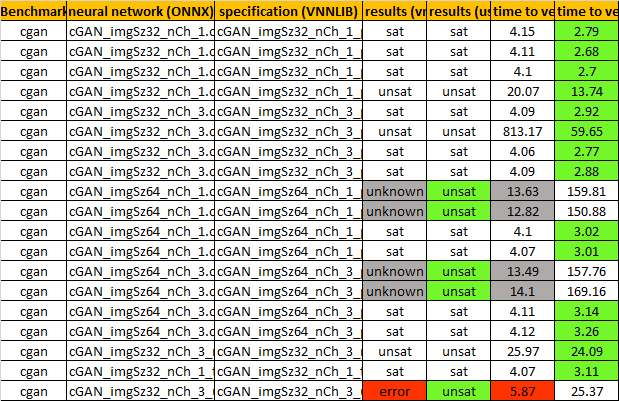
\includegraphics[width=0.8\linewidth]{imagini/interpretare rezultate/NeuralSAT_comp_vs_us.png}
\caption{Comparare rezultate NeuralSAT}
\label{fig:image2} 
\end{figure}
\

Comparând coloanele de \textit{results} am observat faptul că pentru toate instanțele am obținut valori satisfiabile sau nesatisfiabile. În schimb, competiția a obținut în cazul unor instanțe valori de \textit{unknown} si \textit{error}.

Graficul prezentat mai jos\ref{fig:image4}, evidențiază distribuirea timpilor de execuție pentru fiecare instanță în parte. În cadrul graficului de mai jos, se pot observa diferențele dintre timpii de execuție.
\begin{figure}[h]
\centering 
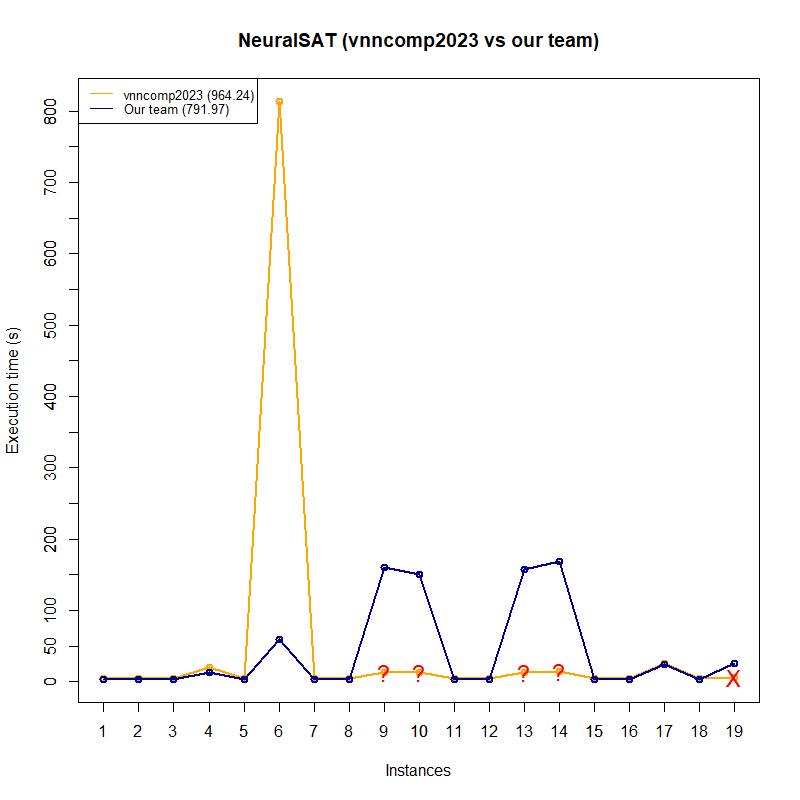
\includegraphics[width=0.8\linewidth]{imagini/interpretare rezultate/NeuralSAT_us_vs_vnncomp2023.png}
\caption{Comparare rezultate NeuralSAT}
\label{fig:image4} 
\end{figure}
\
    \subsection{Compararea rezultatelor obținute pe cele două tool-uri}
    

În urma rulării a tuturor fișierelor atât pentru alpha\_beta\_CROWN, cât și pentru NeuralSAT am obținut un număr de instanțe, pentru care timpul alocat verificării a fost depășit, egal cu 0. Prin urmare nu avem penalități pentru niciunul dintre tool-uri.

Totodată am obținut un Total verified egal cu 8, și un Total falsified egal cu 11 pentru ambele tool-uri. Pentru alpha\_beta\_CROWN rezultatele sunt identice cu cele din competiție. În cazul NeuralSAT, se poate observa că solver-ul
a suferit îmbunătățiri în urma livrărilor constante făcute de dezvoltatori deoarece rezultatele obținute de noi au strâns un scor perfect de 100\%, mult peste cel obținut de solver în cadrul competiției.

\begin{table}[h]
\centering
\begin{tabular}{clcccccc}
\hline
\# & Tool & Verified & Falsified & Fastest & Penalty & Score & Percent \\ \hline
1 & \(\alpha\)-\(\beta\) CROWN & 8 & 11 & 0 & 0 & 190 & 100\% \\
2 & NeuralSAT & 8 & 11 & 0 & 0 & 190 & 100\% \\ \hline
\end{tabular}
\end{table}

Din tabelul de mai jos putem sa ne dam seama(mai mult sau mai puțin) că formula de calculare a scorului este: 

\[
\mathbf{\rightarrow \textbf{Verified} \times 10 + \textbf{Falsified} \times 10 - \textbf{Penalty} \times 150}
\]


Procentajul reprezintă scorul obținut exprimat ca procent din scorul maxim
posibil, oferind o imagine de ansamblu asupra performanței, iar formula de calcul
este:
\[
\mathbf{\frac{\textbf{Score} \times 100}{\textbf{max}(\textbf{Score})}}
\]

\begin{figure}[h]
\centering 
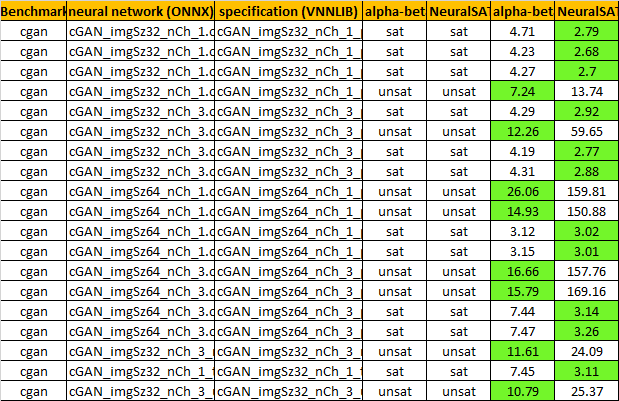
\includegraphics[width=0.8\linewidth]{imagini/interpretare rezultate/alpha-beta-CROWN_vs_NeuralSAT.png}
\caption{Comparare rezultate NeuralSAT vs alpha-beta-CROWN}
\label{fig:image2} 
\end{figure}
\
Analizând datele din tabelul de mai sus, putem observa că în cazul instanțelor cu rezultat satisfiabil (sat) verificatorul NeuralSAT a obținut timpi puțîn mai reduși de execuție decât alpha-beta-CROWN. Pe de altă parte, în cazul instanțelor cu rezultat nesatisfiabil (unsat) timpii de execuție obținuți de alpha-beta-CROWN sunt semnificativ mai reduși decât cei obținuți de NeuralSAT. Acest lucru este evidențiat și in graficul prezentat mai jos, graficul arată distribuirea timpilor de execuție pentru ambele tool-uri, comparând instanța cu instanța.



\begin{figure}[h]
\centering 
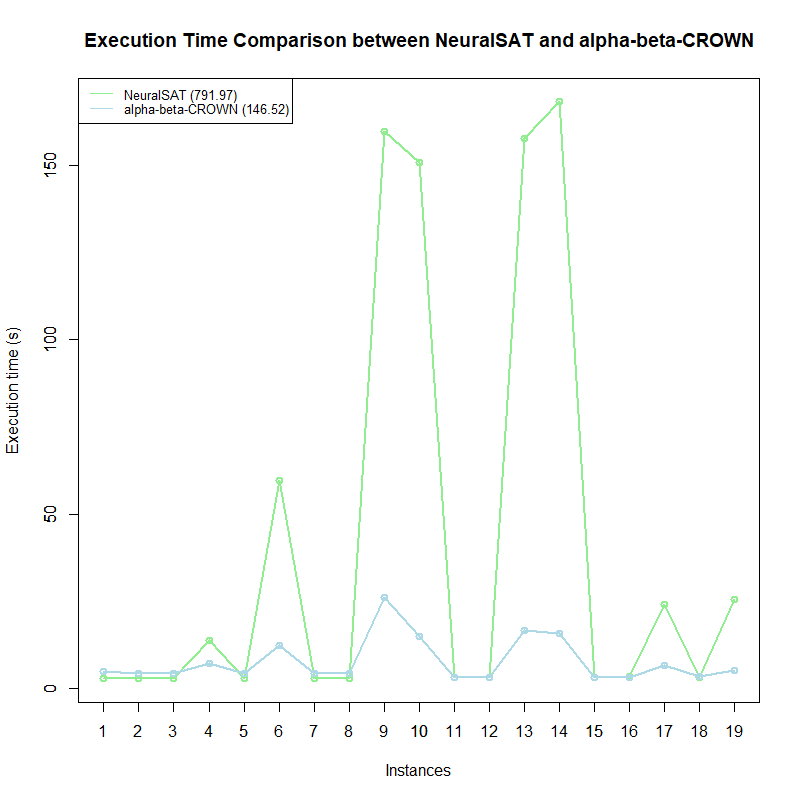
\includegraphics[width=0.8\linewidth]{imagini/interpretare rezultate/Exec_time_comparison.png}
\caption{Comparare rezultate NeuralSAT vs alpha-beta-CROWN}
\label{fig:image2} 
\end{figure}
\
Cel de al doilea grafic prezintă suma timpilor de execuție pe parcursul rulării tuturor celor 19 instanțe pe ambele verificatoare. Din acest grafic se poate trage concluzia că alpha-beta-CROWN este un tool mult mai eficient din punct de vedere a timpului de execuție.

\begin{figure}[h]
\centering 
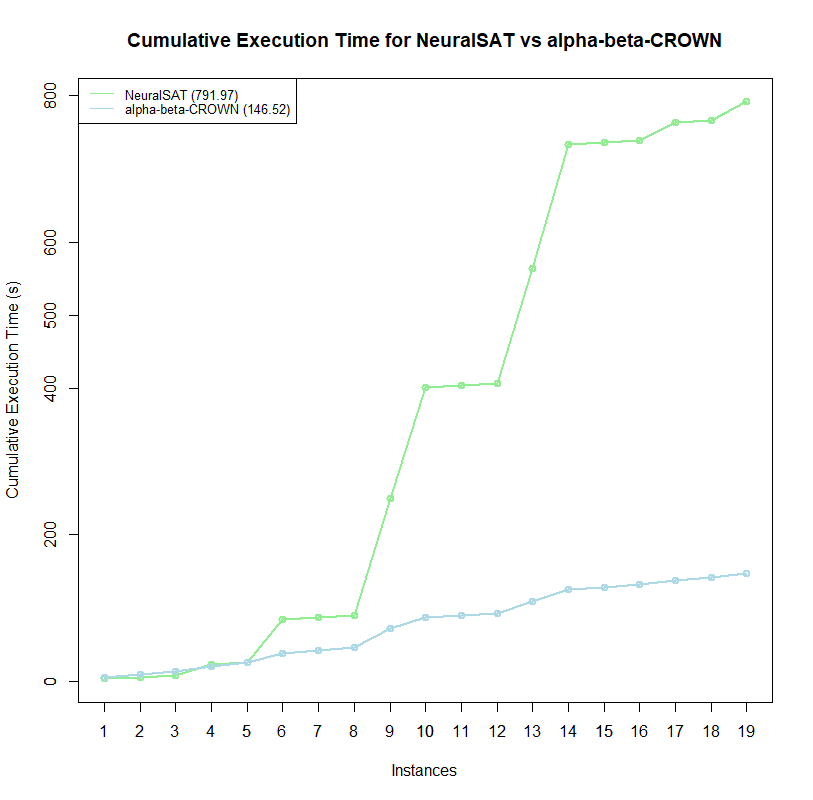
\includegraphics[width=0.8\linewidth]{imagini/interpretare rezultate/cumulative_NeuralSAT_vs_abC.png}
\caption{}
\label{fig:image2} 
\end{figure}
\




%%%%%%%%%%%%%%%%%%%%%%%%%%%%%%%%%%%%%%%%%%%%%%%%%%%%%%%%%%%%%%%%%%%%%%%%%%%%



%%%%%%%%%%%%%%%%%%%%%%%%%%%%%%%%%%%%%%%%%%%%%%%%%%%%%%%%%%%%%%%%%%%%%%%%%%%%
\section{Rețelele neuronale în simularea provocărilor reale}
\hspace{0.5 cm}
Verificarea rețelelor neuronale este o etapă crucială în dezvoltarea și aplicarea modelelor avansate. Aceasta este esențială din mai multe motive importante.

În primul rând, corectitudinea și fiabilitatea rețelelor neuronale sunt imperative. Ele sunt utilizate într-o varietate de domenii, de la medicină și tehnologie până la securitate cibernetică și vehicule autonome. Verificarea ne asigură că aceste rețele funcționează conform așteptărilor, oferind rezultate precise și fiabile într-o gamă largă de situații.

Siguranța reprezintă un alt aspect esențial. În domenii critice precum medicina sau industria automotive, erorile în funcționarea rețelelor neuronale pot avea consecințe grave. Verificarea este necesară pentru a identifica și remedia eventualele vulnerabilități care ar putea pune în pericol sistemul.

În industria auto, utilizarea învățării profunde și a viziunii artificiale pentru generarea de imagini noi joacă un rol esențial. Aceste tehnologii permit generarea de imagini sintetice pentru antrenarea și testarea vehiculelor autonome, simularea diverselor scenarii de conducere și optimizarea sistemelor de vizualizare și senzorilor \cite{googleAppliedDeep}. Ele contribuie la îmbunătățirea siguranței și eficienței în transporturi și la dezvoltarea vehiculelor autonome mai avansate. Utilizarea rețelelor neuronale în generarea de imagini pentru industria auto contribuie prin antrenarea eficientă a algoritmilor, simularea sigură a situațiilor de trafic și optimizarea senzorilor, accelerând dezvoltarea și îmbunătățirea vehiculelor autonome.

De asemenea, verificarea rețelelor neuronale contribuie la prevenirea bias-ului și discriminării. Aceste rețele pot fi influențate de prejudecăți încorporate în datele de antrenament. Prin teste și evaluări riguroase, putem identifica și corecta aceste bias-uri pentru a asigura obiectivitate și corectitudine în rezultatele obținute.
%%%%%%%%%%%%%%%%%%%%%%%%%%%%%%%%%%%%%%%%%%%%%%%%%%%%%%%%%%%%%%%%%%%%%%%%%%%%



%%%%%%%%%%%%%%%%%%%%%%%%%%%%%%%%%%%%%%%%%%%%%%%%%%%%%%%%%%%%%%%%%%%%%%%%%%%%
\section{Concluzii}
%%%%%%%%%%%%%%%%%%%%%%%%%%%%%%%%%%%%%%%%%%%%%%%%%%%%%%%%%%%%%%%%%%%%%%%%%%%%



\bibliography{mybib}
\bibliographystyle{IEEEtran}
\bibliographystyle{alpha}
\addcontentsline{toc}{chapter}{Bibliography}

\end{document}
